
In this section, experiments comparing the Plane-Tree with the Octree in terms of 3D frame or 3D occupancy reconstruction grid compression. Essentially this experiments compares the performance of the Plane-Tree and Octree in 3D occupancy grid compression. \\

The Octree is used for comparison since it is the closest relative of the Plane-Tree and existing methods which use the Octree are presently used in 3D reconstruction research. There is also a 3D implementation of the Interpolating Leaf Quad-Tree \ref{Lincoln13Interpolating} compression algorithm used in the comparison. Being the 3D extension it is therefore referred to as the Interpolating Leaf Octree algorithm (ILOT). \\

In this experiment, Rate-Distortion is measured in PSNR (Peak Signal to Noise Ratio) which is a measurement of the amount of accuracy between the original model and the compressed version for a given algorithm and level of compression. The larger the PSNR, the higher the quality in which the compression system produces for a given bitrate. \\

A Rate-Distortion graph comparing the Plane-Tree, Octree and ILOT is presented in figure \ref{fig:3DReconCompression1}. Results show that for low bit-rates the ILOT outperforms the Octree method. However as higher quality is required, the Octree in turn outperforms the ILOT method. The Plane-Tree algorithm proposed in this work is shown to be dominant compared to both algorithms. For each algorithm, at any bitrate, the Plane-Tree has a much larger Peak-Signal-To-Noise ratio. \\

\begin{figure}[!htb]
\centering
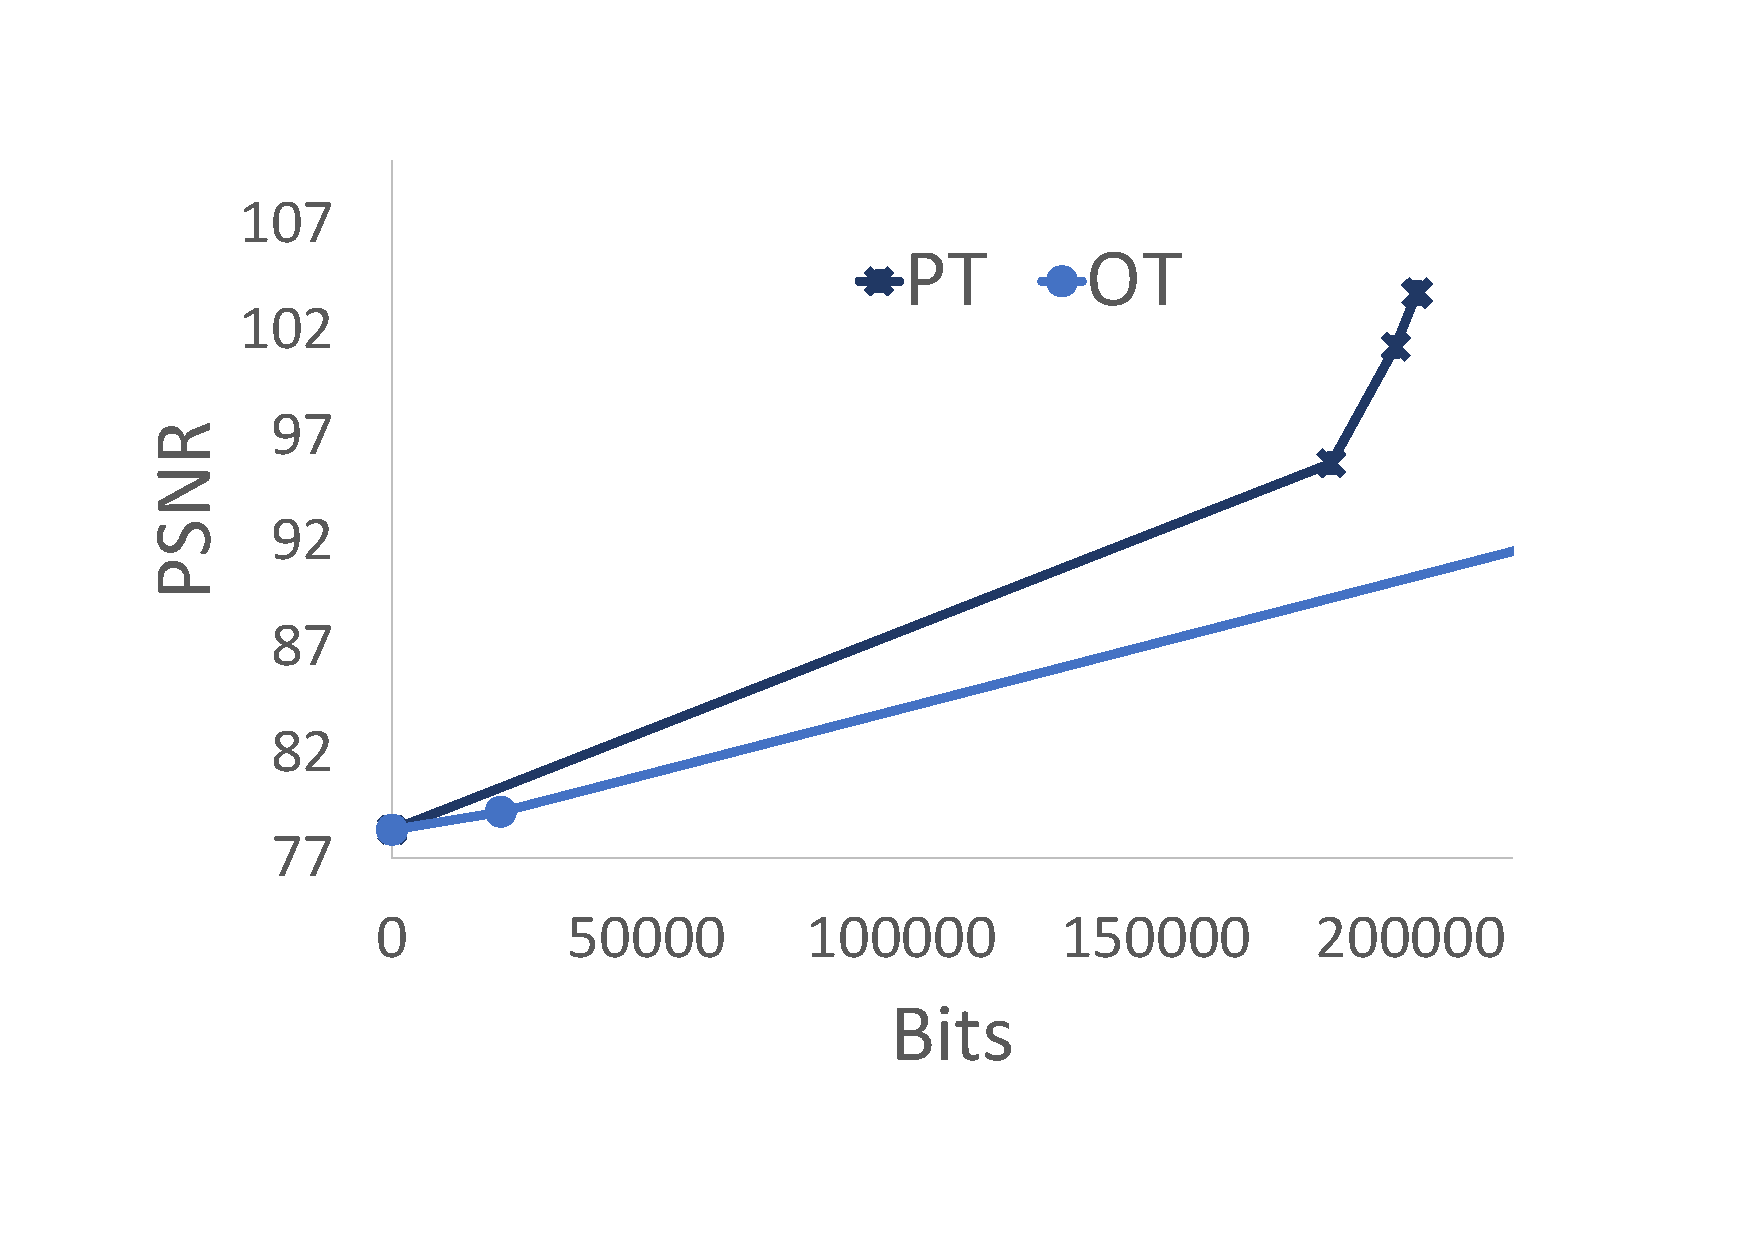
\includegraphics[width=4.0in]{images/results/compression/psnr1}
\caption{PSNR vs Bitrate comparing the ILOT, OT and PT compression methods.}
\label{fig:3DReconCompression1}
\end{figure}

